\documentclass[a4paper,12pt,twoside]{memoir}
\usepackage{btp}    % Use the trainermanual package option (i.e. \usepackage[trainermanual]{btp}) to generate the Trainer's version of the manual
%\usepackage[
%  noinfo,
%  cam,
%  cross,                % crosses as marks
%  a4,
%  width=6.25in,         % the width of the galley
%  height=9.25in,        % the height of the galley
%  center                % actual page is centered on the galley
%]{crop}
% Set some Workshop specific info
\setWorkshopTitle{Introduction to Next Generation Sequencing Hands-on Workshop}
\setWorkshopVenue{}
\setWorkshopDate{}
\setWorkshopAuthor{
Bioplatforms Australia (BPA)\\
The Commonwealth Scientific and Industrial Research Organisation (CSIRO)\\
}

\begin{document}

%
% Workshop Title Page
%
\workshoptitlepage

%
% CC-BY
%
\chapter{Licensing}

This work is licensed under a Creative Commons Attribution 3.0 Unported License and
the below text is a summary of the main terms of the full Legal Code (the full licence) available at
\url{http://creativecommons.org/licenses/by/3.0/legalcode}.

\begin{description}[style=multiline,labelindent=0cm,align=left,leftmargin=1.5cm]
\item[You are free:] \hfill

to copy, distribute, display, and perform the work 

to make derivative works

to make commercial use of the work
  
\item[Under the following conditions:] \hfill

  \textbf{Attribution} - You must give the original author credit.
  
\item[With the understanding that:] \hfill

  \textbf{Waiver} - Any of the above conditions can be waived if you get permission from the
  copyright holder.
  
  \textbf{Public Domain} - Where the work or any of its elements is in the public domain
  under applicable law, that status is in no way affected by the license.
  
  \textbf{Other Rights} - In no way are any of the following rights affected by the license:
  
  \begin{itemize}
    \item Your fair dealing or fair use rights, or other applicable copyright exceptions and limitations;
  
    \item The author's moral rights;
  
    \item Rights other persons may have either in the work itself or in how the work is used, such
    as publicity or privacy rights.
  \end{itemize}
  
  \textbf{Notice} - For any reuse or distribution, you must make clear to others the
  licence terms of this work.
  
\end{description}

\vspace{\fill}

\begin{center}

\includegraphics[height=1cm]{./licences/cc_by.png}
\end{center}

\clearpage

\tableofcontents

\chapter{Workshop Information}
\clearpage

%
% Trainers Page
%
\section{The Trainers}

\newlength{\trainerIconWidth}
\setlength{\trainerIconWidth}{2.0cm}

\begin{table}[H]
  \centering
  \small
  \renewcommand{\arraystretch}{1}
  %\caption{A table arranging  images}
  \rowcolors{1}{gray!25}{white}
  \begin{tabular}{>{\centering\arraybackslash} m{1.1\trainerIconWidth} m{1\textwidth}}
    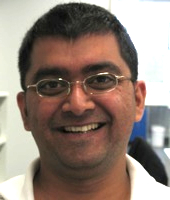
\includegraphics[width=\trainerIconWidth]{graphics/Deshpande.jpg} & 
      \textbf{Dr. Nandan Deshpande}\newline
      
      Postdoctoral Fellow\newline
      The University of New South Wales (UNSW), NSW\newline
      \mailto{n.deshpande@unsw.edu.au}\\
    
    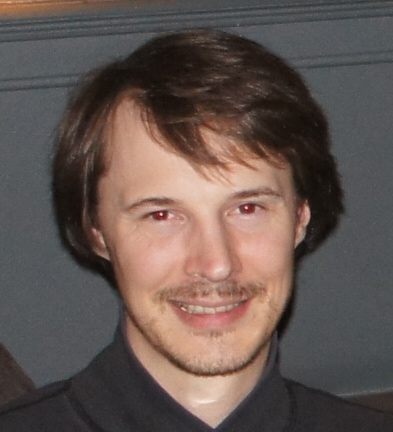
\includegraphics[width=\trainerIconWidth]{graphics/Duesing.jpg} & 
      \textbf{Dr. Konsta Duesing}\newline
      
      Research Team Leader - Statistics \& Bioinformatics\newline
      CSIRO Animal, Food and Health Science, NSW\newline
      \mailto{konsta.duesing@csiro.au}\\
    
    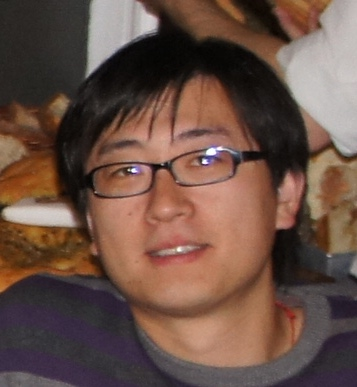
\includegraphics[width=\trainerIconWidth]{graphics/Li.jpg} & 
      \textbf{Dr. Xi (Sean) Li}\newline
      
      Bioinformatics Analyst\newline
      Bioinformatics Core, CSIRO Mathematics, Informatics and Statistics, ACT\newline
      \mailto{sean.li@csiro.au}\\
    
    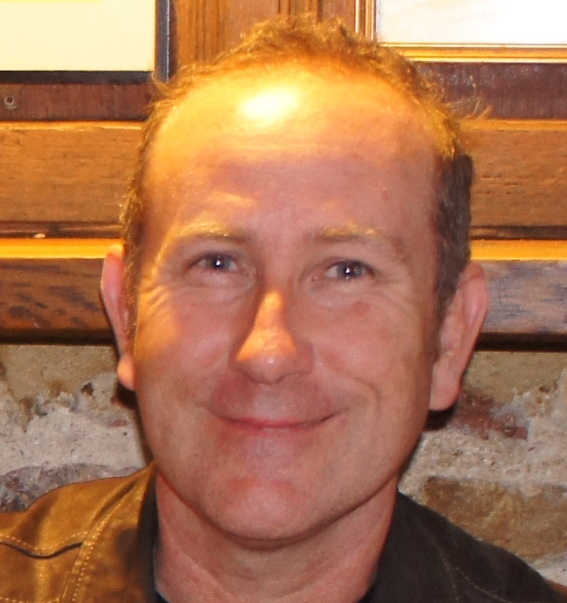
\includegraphics[width=\trainerIconWidth]{graphics/McWilliam.jpg} & 
      \textbf{Mr. Sean McWilliam}\newline
      
      Bioinformatics Analyst\newline
      CSIRO Animal, Food and Health Sciences, QLD\newline
      \mailto{sean.mcwilliam@csiro.au}\\
    
    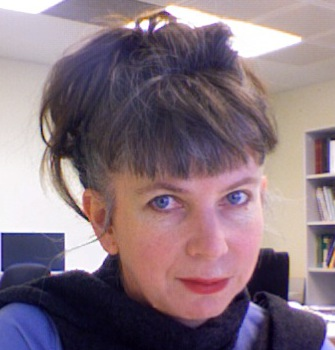
\includegraphics[width=\trainerIconWidth]{graphics/Moolhuijzen.jpg} & 
      \textbf{Dr. Paula Moolhuijzen}\newline
      
      Senior Bioinformatics Officer\newline
      Centre for Comparative Genomics, Murdoch University, WA\newline
      \mailto{pmoolhuijzen@ccg.murdoch.edu.au}\\
    
    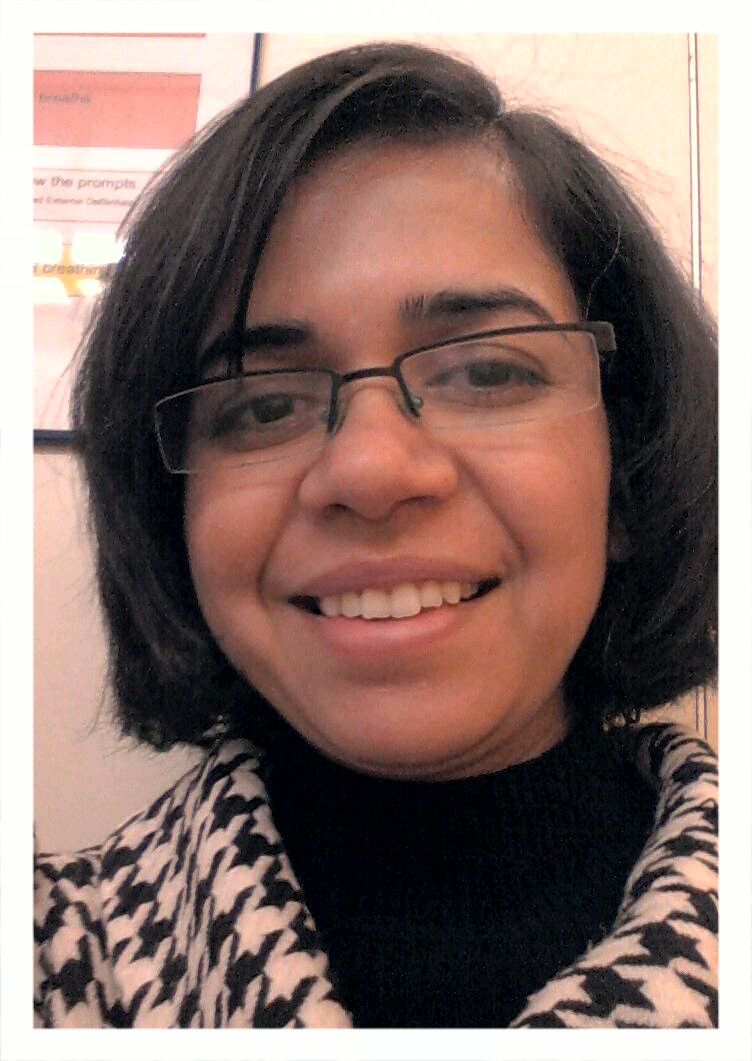
\includegraphics[width=\trainerIconWidth]{graphics/Tyagi.jpg} & 
      \textbf{Dr. Sonika Tyagi}\newline
      
      Senior Bioinformatics Officer\newline
      Australian Genome Research Facility Ltd, The Walter and Eliza Hall Institute, VIC\newline
      \mailto{sonika.tyagi@agrf.org.au}\\
    
    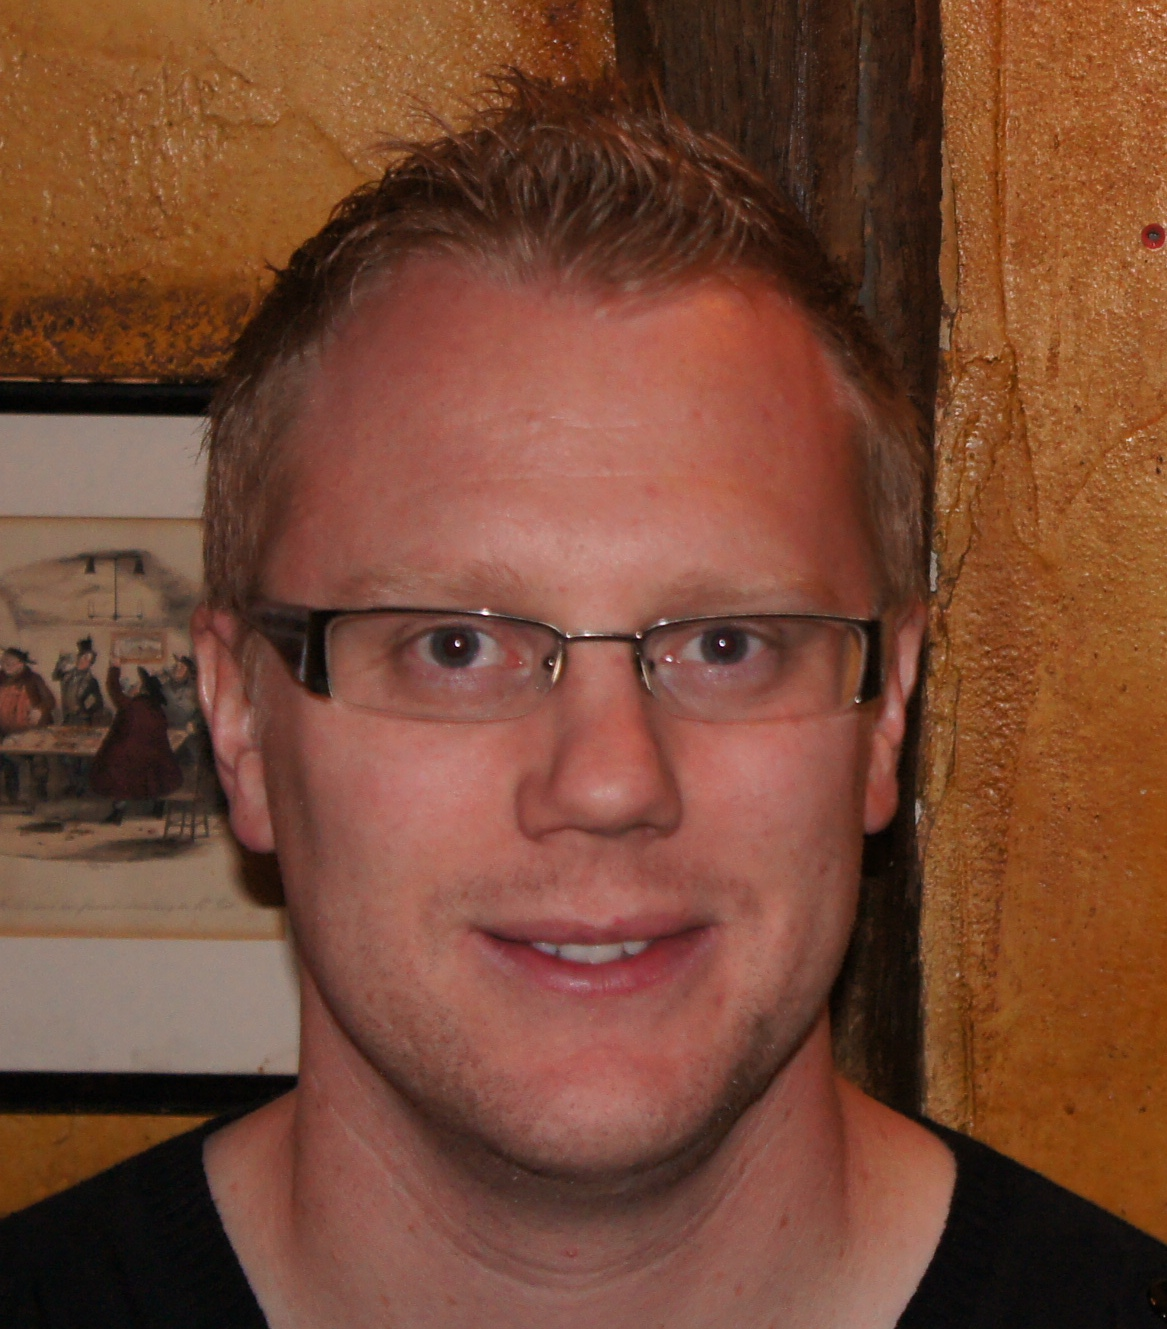
\includegraphics[width=\trainerIconWidth]{graphics/watson-haigh.jpeg} & 
      \textbf{Dr. Nathan S. Watson-Haigh}\newline
      
      Research Fellow in Bioinformatics\newline
      The Australian Centre for Plant Functional Genomics (ACPFG), SA\newline
      \mailto{nathan.haigh@acpfg.com.au}\\
    
    \end{tabular}
  \caption{\label{tab:trainers}}
\end{table}


%
% Workshop Preamble
%
%
% Start: General Information describing the workshop and the structure of the handouts
%
\newpage

% \section{Do's and Don'ts of the Workshop}
% TODO Add do's and don'ts e.g. email, social media etc 

\section{Document Structure}
We have provided you with an electronic copy of the workshop's hands-on tutorial documents.
We have done this for two reasons: 1) you will have something to take away with you at the 
end of the workshop, and 2) you can save time (mis)typing commands on the command line by using
copy-and-paste.

\begin{warning}
While you could fly through the hands-on sessions doing
copy-and-paste you will learn more if you take the time, saved from not having to type all those
commands, to understand what each command is doing!
\end{warning}

The commands to enter at a terminal look something like this:
\begin{lstlisting}
tophat --solexa-quals -g 2 --library-type fr-unstranded -j annotation/Danio_rerio.Zv9.66.spliceSites -o tophat/ZV9_2cells genome/ZV9 data/2cells_1.fastq data/2cells_2.fastq
\end{lstlisting}  

The following icons are used in the margin, throughout the documentation to help you locate:

% TODO limit the use of some icons throughout as some are clearly overused and confuse the eye
\hspace*{.2cm}\vcent{
\includegraphics[height=1cm]{./graphics/info.png}} Important\\
\hspace*{.2cm}\vcent{
\includegraphics[height=1cm]{./graphics/notes.png}} For reference\\
\hspace*{.2cm}\vcent{
\includegraphics[height=1cm]{./graphics/steps.png}} Follow these steps\\
\hspace*{.2cm}\vcent{
\includegraphics[height=1cm]{./graphics/questions.png}} Questions to answer\\
\hspace*{.2cm}\vcent{
\includegraphics[height=1cm]{./graphics/warning.png}} Warning - STOP and read\\
\hspace*{.2cm}\vcent{
\includegraphics[height=1cm]{./graphics/bonus1.png}} Bonus exercise for fast learners\\
\hspace*{.2cm}\vcent{
\includegraphics[height=1cm]{./graphics/bonus2.png}} Advanced exercise for super-fast learners\\

\section{Resources Used}
We have provided you with an environment which contains all the tools and data
you need for the duration of this workshop. However, we also provide details
about the tools and data used by each module at the start of the respective
module documentation.


%
% Start of modules
% Switch chapter styling to module
%
\chapterstyle{module}

%
% QC Module
%
% Define the top matter
\renewcommand{\moduleTitle}{Data Quality}
\renewcommand{\moduleAuthors}{%
  Sonika Tyagi \mailto{sonika.tyagi@agrf.org.au}
} \renewcommand{\moduleContributions}{%
  Nathan S. Watson-Haigh \mailto{nathan.watson-haigh@awri.com.au}%
}

%  Start: Module Title Page
\chapter{\moduleTitle}
\newpage
% End: Module Title Page

\section{Key Learning Outcomes}

After completing this practical the trainee should be able to:
\begin{itemize}
  \item Assess the overall quality of NGS sequence reads
  \item Visualise the quality, and other associated matrices, of reads to decide
        on filters and cutoffs for cleaning up data ready for downstream analysis
  \item Clean up and pre-process the sequences data for further analysis
\end{itemize}

\section{Resources You'll be Using}
 
\subsection{Tools Used}
\begin{description}[style=multiline,labelindent=0cm,align=left,leftmargin=0.5cm]
  \item[FastQC]\hfill\\
  	\url{http://www.bioinformatics.babraham.ac.uk/projects/fastqc/}
  \item[FASTX-Toolkit]\hfill\\
  	\url{http://hannonlab.cshl.edu/fastx_toolkit/}
  \item[Picard]\hfill\\
  	\url{http://picard.sourceforge.net/}
\end{description}

% \subsection{Sources of Data}
% TODO Provide a publically available data set used for this module
% \url{http://www.ebi.ac.uk/ena/data/view/ERR022484}\\
% \url{http://www.ebi.ac.uk/ena/data/view/ERR022485}

\newpage

\section{Introduction}

\begin{note}
Going on a blind date with your read set? For a better understanding of the
consequences please check the data quality!
\end{note}

For the purpose of this tutorial we are focusing only on Illumina sequencing
which uses 'sequence by synthesis' technology in a highly parallel fashion.
Although Illumina high throughput  sequencing provides highly accurate sequence
data, several sequence artefacts, including base calling errors and small
insertions/deletions, poor quality reads and primer/adapter contamination are
quite common in the high throughput sequencing data. The primary errors are
substitution errors. The error rates can vary from 0.5-2.0\% with errors mainly
rising in frequency at the 3' ends of reads.

One way to investigate sequence data quality is to visualize the quality scores
and other metrics in a compact manner to get an idea about the quality of a read
data set. Read data sets can be improved by post processing in different ways
like trimming off low quality bases, cleaning up any sequencing adapters and
removing PCR duplicates. We can also look at other statistics such
as, sequence length distribution, base composition, sequence complexity,
presence of ambiguous bases etc. to assess the overall quality of the data set.
Highly redundant coverage ($>$15X) of the genome can be used to correct sequencing
errors in the reads before assembly and errors. Various k-mer based error
correction methods exist but are beyond the scope of this tutorial.

\section{Prepare the Environment}

\begin{information}
To investigate sequence data quality we will demonstrate tools called FastQC
and FASTX-Toolkit. FastQC will process and present the reports in a visual manner.
Based on the results, the sequence data can be processed using the FASTX-Toolkit.
We will use one data set in this practical, which can be found in the QC
directory on your desktop.
\end{information}

\begin{steps}
Open the Terminal and go to the directory where the data are stored:
\begin{lstlisting}
cd ~/QC/
pwd
\end{lstlisting}

At any time, help can be displayed for FastQC using the following command:
\begin{lstlisting}
fastqc -h
\end{lstlisting}

\end{steps}


\section{Quality Visualisation}

\begin{information}
We have a file for a good quality and bad quality statistics. FastQC generates
results in the form of a zipped and unzipped directory for each input file.
\end{information}

\begin{steps}
Execute the following command on the two files:
\begin{lstlisting}
fastqc -f fastq bad_example.fastq 
fastqc -f fastq good_example.fastq
\end{lstlisting}

View the FastQC report file of the dab data using a web browser such as
firefox.

\begin{lstlisting}
firefox bad_example_fastqc/fastqc_report.html &
\end{lstlisting}

\end{steps}

\begin{note}
The report file will have a Basic Statistics table and various graphs and tables
for different quality statistics. E.g.:
\end{note}

% Table generated by Excel2LaTeX from sheet 'Sheet1'
\begin{table}[H]
  \centering
  \caption{FastQC Basic Statistics table}
    \begin{tabular}{ll}
    \toprule
    Filename & bad\_example.fastq \\
    \midrule
    File type & Conventional base calls \\
    Encoding & Sanger / Illumina 1.9 \\
    Total Sequences & 40000 \\
    Filtered Sequences & 0 \\
    Sequence length & 100 \\
    \%GC  & 48 \\
    \bottomrule
    \end{tabular}%
  \label{tab:badexampleuntrimmed}%
\end{table}%

\begin{figure}[H]
\centering
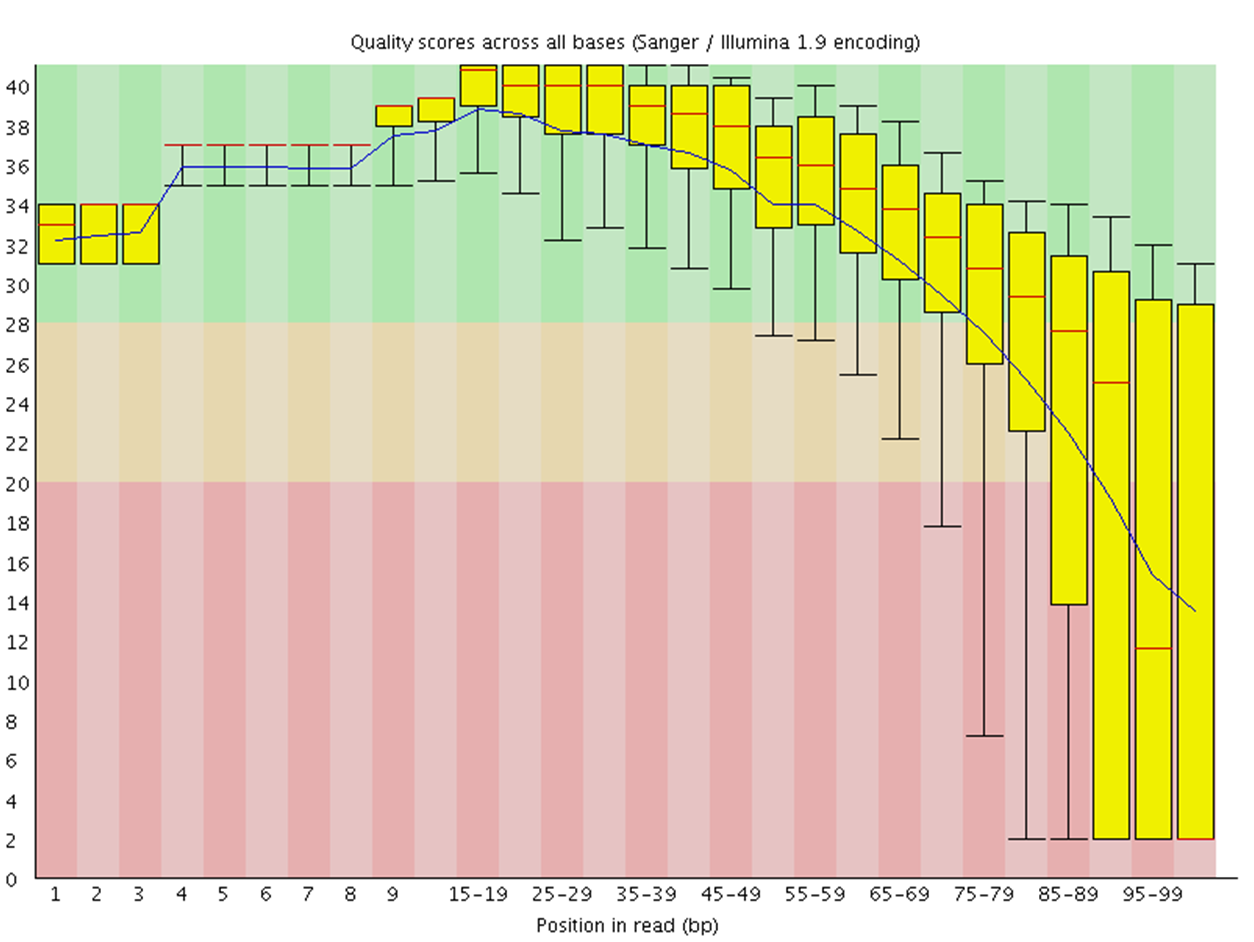
\includegraphics[width=0.8\textwidth]{ngs-qc/bad_example.png}
\caption{Per base sequence quality plot for \texttt{bad\_example.fastq}. Base positions in the reads are shown on x-axis and quality score (Q Score) are shown on the Y-axis}
\label{fig:bad_example_plot}
\end{figure}

\begin{information}
A quality score (or Q-score) expresses an error probability.  In particular, it
serves as a convenient and compact way to communicate very small error
probabilities.
Given an assertion, A, the probability that A is not true, $P(~ A)$, is expressed
by a quality score, $Q(A)$, according to the relationship:
\\\\
$Q(A) =-10 log10(P(\sim A))$
\\\\
Where $P(~ A)$ is the estimated probability of an assertion A being wrong.
The relationship between the quality score and error probability is demonstrated
with the following table:

% Table generated by Excel2LaTeX from sheet 'Sheet1'
\begin{table}[H]
  \centering
  \caption{Error probabilities associated with various quality (Q) values}
    \begin{tabular}{rr}
    \toprule
    \textbf{Quality score, Q(A)} & \textbf{Error probability, P($\sim$A)} \\
    \midrule
    10    & 0.1 \\
    20    & 0.01 \\
    30    & 0.001 \\
    40    & 0.0001 \\
    \bottomrule
    \end{tabular}%
  \label{tab:addlabel}%
\end{table}%

\end{information}

\begin{questions}
How many sequences were there in your file? What is the read length?
\begin{answer}
40,000. read length=100bp
\end{answer}

Does the quality score values vary throughout the read length?
(hint: look at the 'per base sequence quality plot')
\begin{answer}
Yes. Quality scores are dropping towards the end of the reads.
\end{answer}

What is the quality score range you see?
\begin{answer}
2-40
\end{answer}

At around which position do the scores start falling below Q20? 
\begin{answer}
Around 80 bp position
\end{answer}


How can we trim the reads to filter out the low quality data?
\begin{answer}
By trimming off the bases after a fixed position of the read. or by trimming off bases based on the quality score.
\end{answer}
\end{questions}

\begin{bonus}
\subsection{Good Quality Data}
View the FastQC report files fastqc\_report.html to see examples of a good
quality data and compare the quality plot with that of the bad\_example\_fastqc.

\begin{lstlisting}
firefox good_example_fastqc/fastqc_report.html &
\end{lstlisting}
\end{bonus}

\begin{note}
Sequencing errors can complicate the downstream analysis, which normally
requires that reads be aligned to each other (for genome assembly) or to a
reference genome (for detection of mutations). Sequence reads containing errors
may lead to ambiguous paths in the assembly or improper gaps. In variant
analysis projects sequence reads are aligned against the reference genome. The
errors in the reads may lead to more mismatches than expected from
mutations alone. But if these errors can be removed or corrected, the read
alignments and hence the variant detection will improve. The assemblies will also
improve after pre-processing the reads with errors.
\end{note}

\section{Read Trimming}
Read trimming can be done in a variety of different ways. Choose a method
which best suits your data. Here we are giving examples of fixed-length trimming
and quality-based trimming.

\subsection{Fixed Length Trimming}
Low quality read ends can be trimmed using a fixed-length timmer. We will use the
\texttt{fastx\_trimmer} from the FASTX-Toolkit. Usage message to find out various options
you can use with this tool. Type \fonttt{fastx\_trimmer -h} at anytime to display help.

\begin{steps}
We will no do fixed-length trimming of the \texttt{bad\_example.fastq} file
using the following command.
\begin{lstlisting}
cd ~/QC
fastx_trimmer -h
fastx_trimmer -Q 33 -f 1 -l 80 -i bad_example.fastq -o bad_example_trimmed01.fastq
\end{lstlisting}
\end{steps}

\begin{note}
We used the following options in the command above:
\begin{description}[style=multiline,labelindent=0cm,align=right,leftmargin=\descriptionlabelspace,rightmargin=1.5cm,font=\ttfamily]
 \item[-Q 33] Indicates the input quality scores are Phred+33 encoded
 \item[-f] First base to be retianed in the output
 \item[-l] Last base to be retained in the output
 \item[-i] Input fastq file name
 \item[-o] Output file name
\end{description}
\end{note}

\begin{steps}
Run FastQC on the trimmed file and visualise the quality scores of the trimmed file.
\begin{lstlisting}
fastqc -f fastq bad_example_trimmed01.fastq
firefox bad_example_trimmed01_fastqc/fastqc_report.html &
\end{lstlisting}

The output should look like:

\begin{table}[H]
  \centering
  \caption{FastQC Basic Statistics table}
    \begin{tabular}{ll}
    \toprule
    Filename & bad\_example\_trimmed01.fastq\\
    \midrule
    File type & Conventional base calls\\
    Encoding & Sanger / Illumina 1.9\\
    Total Sequences & 40000\\
    Filtered Sequences & 0\\
    Sequence length & 80\\
    \%GC & 48\\
    \bottomrule
    \end{tabular}%
  \label{tab:badexampletrimmed}%
\end{table}%

\begin{figure}[H]
\centering
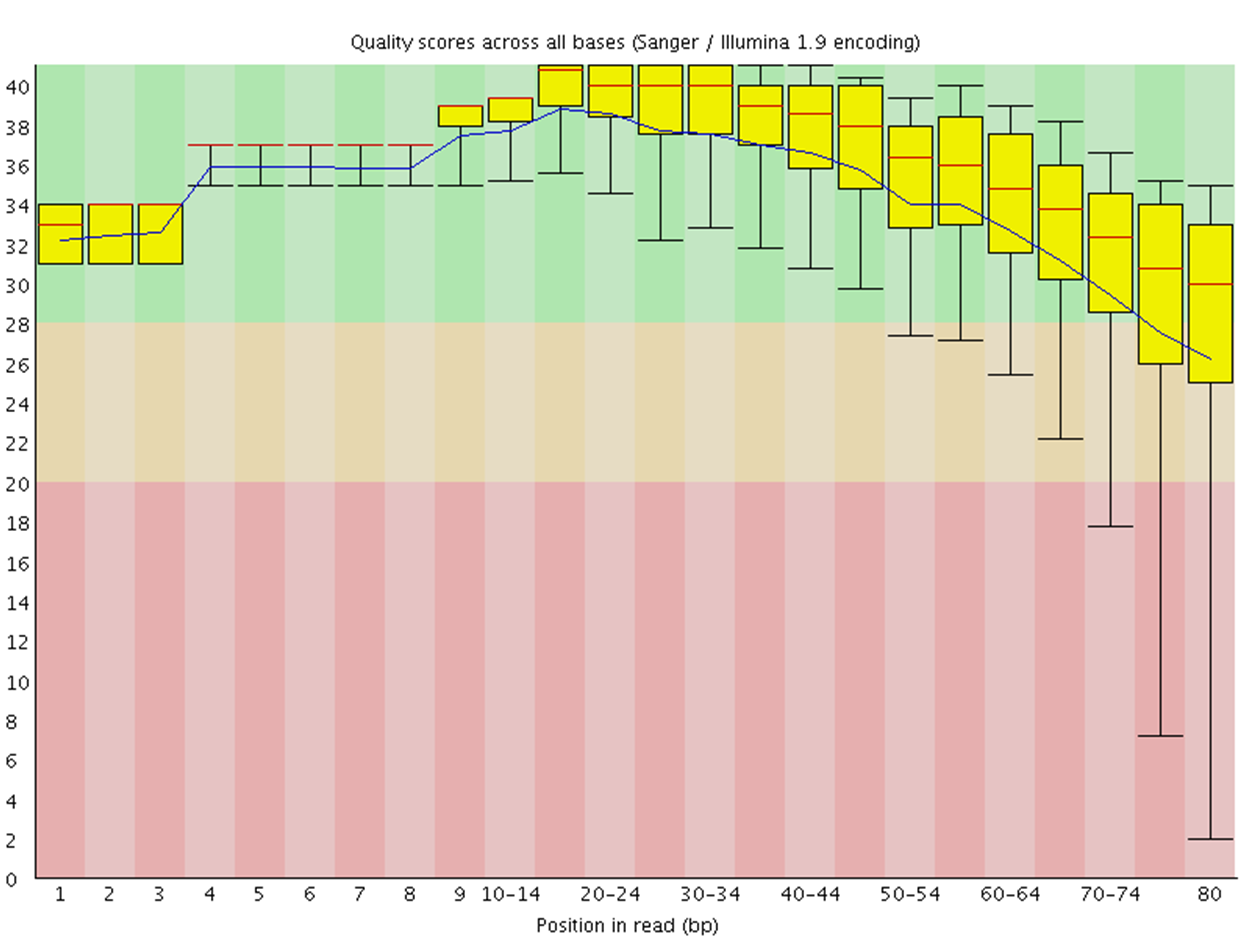
\includegraphics[width=0.8\textwidth]{ngs-qc/bad_example_trimmed_to_80bp.png}
\caption{Per base sequence quality plot for the fixed-length trimmed \texttt{bad\_example.fastq} reads. Base positions in the reads are shown on x-axis and quality score (Q Score) are shown on the Y-axis}
\label{fig:bad_example_trimmed_plot}
\end{figure}

\end{steps}

\begin{questions}
What values would you use for \texttt{-f} if you wanted to trim off 10 bases at
the 5' end of the reads?
\begin{answer}
\texttt{-f 11}
\end{answer}
\end{questions}

\subsection{Quality Based Trimming}
Base call quality scores can also be used to dynamically determine the trim points for each read. A quality
score threshold and minimum read length following trimming can be used to remove low
quality data.

\begin{steps}
Run the following command to quality trim your data:
\begin{lstlisting}
cd ~/QC
fastq_quality_trimmer -h
fastq_quality_trimmer -Q 33 -t 20 -l 50 -i bad_example.fastq -o bad_example_quality_trimmed.fastq
\end{lstlisting}
\end{steps}

\begin{steps}
Run FastQC on the quality trimmed file and visualise the quality scores.

\begin{lstlisting}
fastqc -f fastq bad_example_quality_trimmed.fastq
firefox bad_example_quality_trimmed_fastqc/fastqc_report.html &
\end{lstlisting}

The output should look like:

\begin{table}[H]
  \centering
  \caption{FastQC Basic Statistics table}
    \begin{tabular}{ll}
    \toprule
    Filename & bad\_example\_quality\_trimmed.fastq\\
    \midrule
    File type & Conventional base calls\\
    Encoding & Sanger / Illumina 1.9\\
    Total Sequences & 38976\\
    Filtered Sequences & 0\\
    Sequence length & 50-100\\
    \%GC & 48\\
    \bottomrule
    \end{tabular}%
  \label{tab:badexamplequalitytrimmed}%
\end{table}%

\begin{figure}[H]
\centering
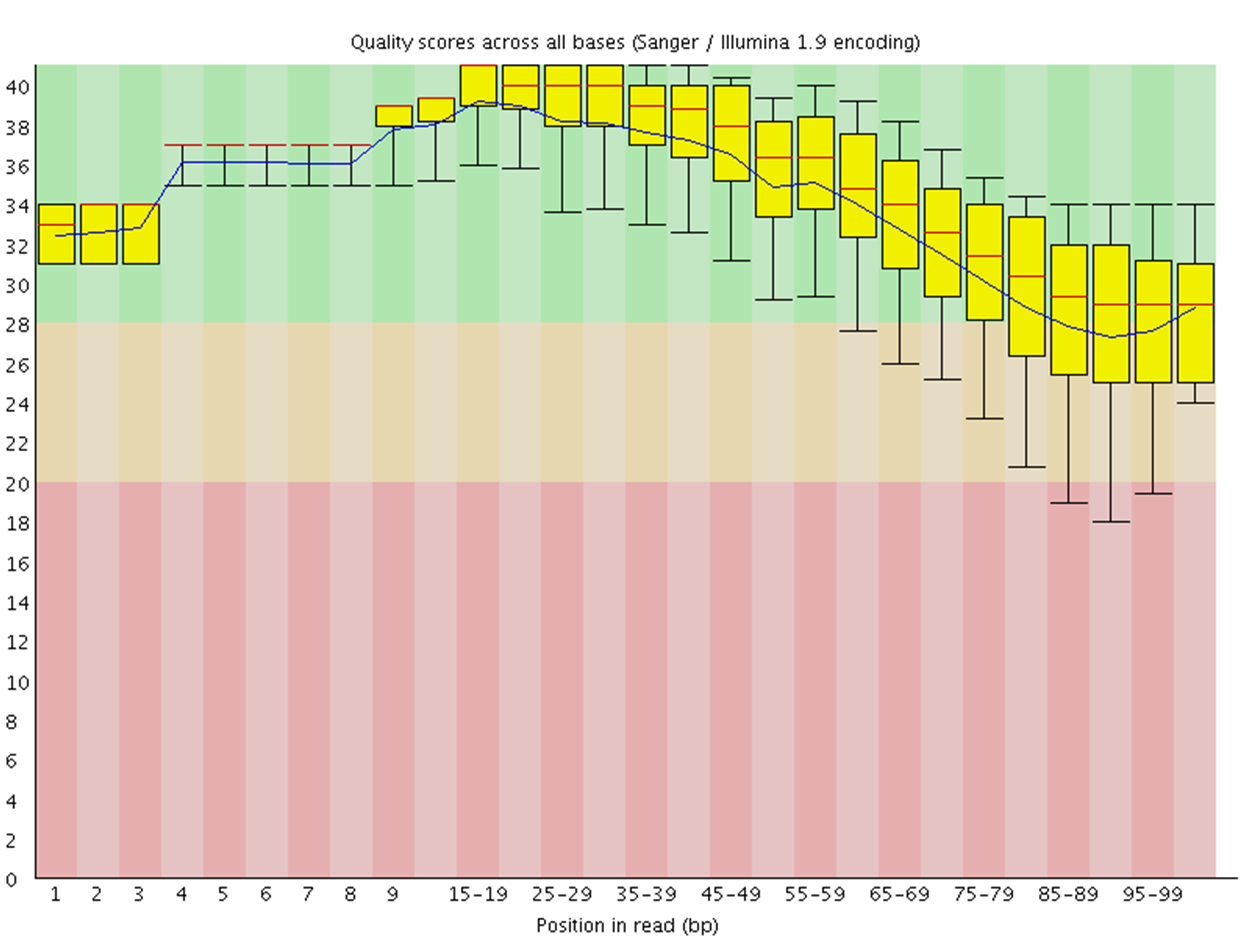
\includegraphics[width=0.8\textwidth]{ngs-qc/bad_example_quality_trimmed.png}
\caption{Per base sequence quality plot for the quality-trimmed \texttt{bad\_example.fastq} reads. Base positions in the reads are shown on x-axis and quality score (Q Score) are shown on the Y-axis}
\label{fig:bad_example_quality_trimmed_plot}
\end{figure}

\end{steps}

\begin{questions}
How did the quality score range change with two types of trimming?
\begin{answer}
Some poor quality bases (Q $<$20) are still present at the 3' end of the
fixed-length trimmed reads. It also removes bases that are good quality.

Quality-based trimming retains the 3' ends of reads which have good quality
scores.
\end{answer}

Did the number of total reads change after two types of trimming?
\begin{answer}
Quality trimming discarded $>$1000 reads. However, We retain a lot of maximal
length reads which have good quality all the way to the ends.
\end{answer}

What reads lengths were obtained after quality based trimming?
\begin{answer}
50-100

Reads $<$50 bp, following quality trimming, were discarded.
\end{answer}

Did you observe adapter sequences in the data?
\begin{answer}
No. (Hint: look at the overrepresented sequences.
\end{answer}

\end{questions}

\begin{advanced}
\subsection{Adapter Clipping}
Sometime sequence reads may end up getting the leftover of adapters and primers
used in the sequencing process. It's good practice to screen your data for
these possible contaminations for more sensitive alignment and assembly based
analysis.

\begin{note}
This is particularly important when read lengths can be longer than the
molecules being sequenced. For example when sequencing miRNAs.
\end{note}

Various QC tools are available to screen and/or clip these adapter/primer
sequences from your data. (e.g. FastQC, fastx, cutadapt).

\begin{steps}
Here we are demonstrating \texttt{fastx\_clipper} to trim a given adapter
sequence.

\begin{lstlisting}
cd ~/QC
fastx_clipper -h
fastx_clipper -v -Q 33 -l 20 -M 15 -a GATCGGAAGAGCGGTTCAGCAGGAATGCCGAG -i bad_example.fastq -o bad_example_clipped.fastq
\end{lstlisting}
\end{steps}

\begin{note}
An alternative tool, not installed on this system, for adapter clipping is
\texttt{fastq-mcf}. A list of adapters is provided in a text file. For more
information, see Fastqmcf at \url{http://code.google.com/p/ea-utils/wiki/FastqMcf}.
\end{note}

\subsection{Removing Duplicates}
Duplicate reads are the ones having the same start and end coordinates. This
may be the result of technical duplication (too many PCR cycles), or
over-sequencing (very high fold coverage). It is very important to put the
duplication level in context of your experiment. For example, duplication level
in targeted or re-sequencing projects may mean something different in RNA-seq
experiments. In RNA-seq experiments oversequencing is usually necessary when
detecting low abundance transcripts.

\begin{information}
The duplication level computed by FastQC is based on sequence identity at the
end of reads. Another tool, Picard, determines duplicates based on identical
start and end positions in SAM/BAM alignment files.

\textbf{We will not cover Picard but
provide the following for your information.}

Picard is a suite of tools for performing many common tasks with SAM/BAM format
files. For more information see the Picard website and information about the
various command-line tools available:

\url{http://picard.sourceforge.net/command-line-overview.shtml}
\end{information}

\begin{information}
Picard 1.69 is installed on this system in \texttt{/usr/share/java/picard-1.69/}

One of the Picard tools (MarkDuplicates) can be used to analyse and remove
duplicates from the raw sequence data. The input for Picard is a sorted
alignment file in BAM format. Short read aligners such as, bowtie, BWA and tophat
can be used to align FASTQ files against a reference genome to generate
SAM/BAM alignment format.
\end{information}

\begin{steps}
Interested users can use the following general command to run the
MarkDuplicates tool at their leisure and only need to provide a BAM file for
INPUT:


\begin{lstlisting}
cd ~/QC
java -jar /usr/share/java/picard/MarkDuplicates.jar INPUT=<alignment_file.bam> VALIDATION_STRINGENCY=LENIENT OUTPUT=alignment_file.dup METRICS_FILE=alignment_file.matric ASSUME_SORTED=true REMOVE_DUPLICATES=true

\end{lstlisting}
\end{steps}

\end{advanced}


%
% Alignment Module
%
% Define the top matter
\renewcommand{\moduleTitle}{Read Alignment}
\renewcommand{\moduleAuthors}{%
  Myrto Kostadima \mailto{kostadim@ebi.ac.uk}
} \renewcommand{\moduleContributions}{%
  Xi Li \mailto{sean.li@csiro.au}%
}

%  Start: Module Title Page
\chapter{\moduleTitle}
\newpage
% End: Module Title Page

\section{Key Learning Outcomes}

After completing this practical the trainee should be able to:
%TODO
\begin{itemize}
  \item Perform the simple NGS data alignment task against one interested reference data \\
  \item Interpret and manipulate the mapping output using samtools \\
  \item Visualise the alignment via a standard genome browser, e.g. IGV browser \\
\end{itemize}
\section{Resources You'll be Using}
 
\subsection{Tools Used}
\begin{description}[style=multiline,labelindent=0cm,align=left,leftmargin=0.5cm]
  \item[Bowtie]\hfill\\
  	\url{http://bowtie-bio.sourceforge.net/index.shtml}
  \item[Bowtie 2]\hfill\\
  	\url{http://bowtie-bio.sourceforge.net/bowtie2/index.shtml}
  \item[Samtools]\hfill\\
  	\url{http://picard.sourceforge.net/}
  \item[BEDTools]\hfill\\
  	\url{http://code.google.com/p/bedtools/}
  \item[UCSC tools]\hfill\\
  	\url{http://hgdownload.cse.ucsc.edu/admin/exe/}  
  \item[IGV genome browser]\hfill\\
  	\url{http://www.broadinstitute.org/igv/}
\end{description}

\subsection{Sources of Data}
  \url{http://www.ebi.ac.uk/arrayexpress/experiments/E-GEOD-11431}
% \url{http://www.ebi.ac.uk/ena/data/view/ERR022484}\\
% \url{http://www.ebi.ac.uk/ena/data/view/ERR022485}

\clearpage

\section{Introduction}

\begin{information}
The goal of this hands-on session is to perform an unspliced alignment for a
small subset of raw reads. We will align raw sequencing data to the mouse genome
using \emph{Bowtie} and then we will manipulate the SAM output in order to
visualize the alignment on the \emph{IGV browser}.
\end{information}

\section{Prepare the Environment}

\begin{information}
We will use one data set in this practical, which can be found in the \texttt{ChIP-seq}
directory on your desktop.
\end{information}

\begin{steps}
Open the Terminal.

First, go to the right folder, where the data are stored.
\begin{lstlisting}
cd ~/ChIP-seq
\end{lstlisting}

\begin{information}
The \texttt{.fastq} file that we will align is called \texttt{Oct4.fastq}. This
file is based on Oct4 ChIP-seq data published by Chen et al. (2008). For the
sake of time, we will align these reads to a single mouse chromosome.
\end{information}
\end{steps}

\section{Alignment}

\begin{information}
You already know that there are a number of competing tools for short read
alignment, each with its own set of strengths, weaknesses, and caveats. Here we
will try \emph{Bowtie}, a widely used ultrafast, memory efficient short read
aligner.
\end{information}

\begin{steps}
\emph{Bowtie} has a number of parameters in order to perform the alignment. To
view them all type

\begin{lstlisting}
bowtie --help
\end{lstlisting}

\emph{Bowtie} uses indexed genome for the alignment in order to keep its memory
footprint small. Because of time constraints we will build the index only for
one chromosome of the mouse genome. For this we need the chromosome sequence in
FASTA format. This is stored in a file named \texttt{mm9}, under the subdirectory
\texttt{bowtie\_index}.

The indexed chromosome is generated using the command:

\begin{lstlisting}
bowtie-build bowtie_index/mm9.fa bowtie_index/mm9
\end{lstlisting}

This command will output 6 files that constitute the index. These files that
have the prefix \texttt{mm9} are stored in the \texttt{bowtie\_index}
subdirectory. To view if they files have been successfully created type:

\begin{lstlisting}
ls -l bowtie_index
\end{lstlisting}
\end{steps}

\begin{information}
Now that the genome is indexed we can move on to the actual alignment. The first
argument for bowtie is the basename of the index for the genome to be searched;
in our case is \texttt{mm9}. We also want to make sure that the output is in SAM
format using the \texttt{-S} parameter. The last argument is the name of the
FASTQ file.
\end{information}

\begin{steps}
Align the Oct4 reads using Bowtie: 

\begin{lstlisting}
bowtie bowtie_index/mm9 -S Oct4.fastq > Oct4.sam
\end{lstlisting}

The above command outputs the alignment in SAM format and stores them in the
file \texttt{Oct4.sam}.
\end{steps}

\begin{note}
In general before you run \emph{Bowtie}, you have to know which encoding your FASTQ files
have. The available FASTQ encodings for bowtie are:

\begin{description}[style=multiline,labelindent=0cm,align=right,leftmargin=\descriptionlabelspace,rightmargin=1.5cm,font=\ttfamily]
 \item[--phred33-quals] Input quals are Phred+33 (default).
 \item[--phred64-quals] Input quals are Phred+64 (same as \texttt{--solexa1.3-quals}).
 \item[--solexa-quals] Input quals are from GA Pipeline ver. $<$ 1.3.
 \item[--solexa1.3-quals] Input quals are from GA Pipeline ver. $\geq$ 1.3.
 \item[--integer-quals] Qualities are given as space-separated integers (not ASCII).
\end{description}

The FASTQ files we are working with are Sanger encoded (Phred+33), which is the
default for \emph{Bowtie}.

\emph{Bowtie} will take 2-3 minutes to align the file. This is fast compared to
other aligners which sacrifice some speed to obtain higher sensitivity.
\end{note}

\begin{steps}
Look at SAM format by typing:

\begin{lstlisting}
head -n 10 Oct4.sam
\end{lstlisting}
\end{steps}

\begin{questions}
Can you distinguish between the header of the SAM format and the actual alignments?
\begin{answer}
%TODO
The header line starts with the letter `@', i.e.: 

\begin{tabular}{llll}
@HD & VN:1.0 & SO:unsorted & \\
@SQ & SN:chr1 & LN:197195432 & \\
@PG & ID:Bowtie &      VN:0.12.8  & CL:``bowtie bowtie\_index/mm9 -S Oct4.fastq'' \\
\end{tabular}

While, the actual alignments start with read id, i.e.:

\begin{tabular}{llll}
SRR002012.45 & 0 & chr1 & etc \\
SRR002012.48 & 16 & chr1 & etc \\
\end{tabular}
\end{answer}

What kind of information does the header provide?
\begin{answer}
%TODO
1. @HD: Header line; VN: Format version; SO: the sorting order of alignment.
2. @SQ: Reference sequence information; SN: reference sequence name; LN: reference sequence length.
3. @PG: Read group information; ID: Read group identifier; VN: Program version; CL: the command line that produces the alignment.
\end{answer}

To which chromosome are the reads mapped? 
\begin{answer}
%TODO
Chromosome 1.
\end{answer}
\end{questions}

\section{Manipulate SAM output}

\begin{note}
SAM files are rather big and when dealing with a high volume of NGS data,
storage space can become an issue. As we have already seen, we can convert SAM
to BAM files (their binary equivalent that are not human readable) that occupy
much less space.
\end{note}

\begin{steps}
Convert SAM to BAM using \emph{samtools} and store the output in the file
\texttt{Oct4.bam}. You have to instruct \emph{samtools} that the input is in SAM
format (\texttt{-S}), the output should be in BAM format (\texttt{-b}) and that
you want the output to be stored in the file specified by the \texttt{-o}
option:

\begin{lstlisting}
samtools view -bSo Oct4.bam Oct4.sam
\end{lstlisting}
\end{steps}

\begin{advanced}
Compute simple stats of the alignment using \emph{samtools}:

\begin{lstlisting}
samtools flagstat Oct4.bam
\end{lstlisting}
\end{advanced}

\section{Visualize alignments in IGV}

\begin{information}
\emph{IGV} is a stand-alone genome browser. Please check their website
(\url{http://www.broadinstitute.org/igv/}) for all the formats that \emph{IGV}
can display. For our visualization purposes we will use the BAM and bigWig
formats.
\end{information}

\begin{note}
When uploading a BAM file into the genome browser, the browser will look for the
index of the BAM file in the same folder where the BAM files is. The index file
should have the same name as the BAM file and the suffix \texttt{.bai}. Finally, to
create the index of a BAM file you need to make sure that the file is sorted
according to chromosomal coordinates.
\end{note}

\begin{steps}
Sort alignments according to chromosome position and store the result in the
file with the prefix \texttt{Oct4.sorted}:

\begin{lstlisting}
samtools sort Oct4.bam Oct4.sorted
\end{lstlisting}

Index the sorted file.

\begin{lstlisting}
samtools index Oct4.sorted.bam
\end{lstlisting}

The indexing will create a file called \texttt{Oct4.sorted.bam.bai}. Note that
you don't have to specify the name of the index file when running samtools.
\end{steps}

\begin{note}
Another way to visualize the alignments is to convert the BAM file into a bigWig
file. The bigWig format is for display of dense, continuous data and the data
will be displayed as a graph. The resulting bigWig files are in an indexed
binary format.
\end{note}

\begin{steps}
The BAM to bigWig conversion takes place in two steps. Firstly, we convert the
BAM file into a bedgraph, called \texttt{Oct4.bedgraph}, using the tool
\texttt{genomeCoverageBed} from \emph{BEDTools}:

\begin{lstlisting}
genomeCoverageBed -bg -ibam Oct4.sorted.bam -g bowtie_index/mouse.mm9.genome > Oct4.bedgraph
\end{lstlisting}

Then we convert the bedgraph into a binary graph, called \texttt{Oct4.bw}, using the
tool \texttt{bedGraphToBigWig} from the \emph{UCSC} tools:

\begin{lstlisting}
bedGraphToBigWig Oct4.bedgraph bowtie_index/mouse.mm9.genome Oct4.bw
\end{lstlisting}
\end{steps}

\begin{note}
Both of the commands above take as input a file called \texttt{mouse.mm9.genome} that
is stored under the subdirectory \texttt{bowtie\_index}. These genome files are
tab-delimited and describe the size of the chromosomes for the organism of
interest. When using the UCSC Genome Browser, Ensembl, or Galaxy, you typically
indicate which species/genome build you are working. The way you do this for
\emph{BEDTools} is to create a ``genome'' file, which simply lists the names of
the chromosomes (or scaffolds, etc.) and their size (in basepairs).

\emph{BEDTools} includes pre-defined genome files for human and mouse in the
\texttt{genomes} subdirectory included in the \emph{BEDTools} distribution.
\end{note}

\begin{steps}
Now we will load the data into the IGV browser for visualization. In order to
launch IGV double click on the IGV 2.1 icon on your Desktop. Ignore any warnings
and when it opens you have to load the genome of interest.

On the top left of your screen choose from the drop down menu \texttt{Mus musculus
(mm9)}. Then in order to load the desire files go to:

\begin{lstlisting}
File > Load from File
\end{lstlisting}

On the pop up window navigate to Desktop $>$ ChIP-seq folder and select the file
\texttt{Oct4.sorted.bam}.

Repeat these steps in order to load \texttt{Oct4.bw} as well.

Select chr1 from the drop down menu on the top left. Right click on the name of
\texttt{Oct4.bw} and choose Maximum under the Windowing Function. Right click again and
select Autoscale.

In order to see the aligned reads of the BAM file, you need to zoom in to a
specific region. For example, look for gene \texttt{Lemd1} in the search box.
\end{steps}

\begin{questions}
What is the main difference between the visualization of BAM and bigWig files?
\begin{answer}
%TODO
The actual alignment of reads that stack to a particular region can be displayed using the information stored in a BAM format.
The bigWig format is for display of dense, continuous data that will be displayed in the Genome Browser as a graph.
\end{answer}
\end{questions}

Using the \texttt{+} button on the top right zoom in more to see the details of the alignment.

\begin{questions}
What do you think the different colors mean?
\begin{answer}
%TODO
The different color represents four nucleotides, e.g. blue is Cytidine (C), red is Thymidine (T).
\end{answer}
\end{questions}

\section{Practice}
In the ChIP-seq folder you will find another \texttt{.fastq} file called
\texttt{gfp.fastq}. Follow the above described analysis for this dataset as well.



%
% End of modules
% Switch back to normal workshop chapter styling
%
\chapterstyle{workshop}



\chapter{Post-Workshop Information}
\clearpage
%
% Access to Computational Resources
%
\section{Access to Computational Resources}

By the end of the workshop we hope you're thinking one or more of the following:

\begin{itemize}
\item I'm interested in dabbling some more during my day-job!
\item How do I access a Linux box like the one I've been using in the workshop -
I \emph{really} don't want the hassle of setting this all up myself!
\item I'm hooked! I \emph{really} want to get down and dirty with NGS data! What
computational resources do I need, what do I have access to and how do I access
them?
\end{itemize}

We're ecstatic you're thinking this way and want to help guide you! However, lets
take this one step at a time.

The quickest way to dabble is to use a clone of the operating system (OS) you've
been using during this workshop. That means you'll have hassle-free access to a
plethora of pre-installed, pre-configured bioinformatics tools. You could even set it
up to contain a copy of all the workshop data and handouts etc to go through the
hands-on practicals in your own time!

We have created an image file (approx. 10 GBytes in size) of the NGS Training OS for you to
use as you wish:
\\\\
%\url{https://swift.rc.nectar.org.au:8888/v1/AUTH_809/NGSImage/NGSTrainingV1.0.vdi}
\url{https://swift.rc.nectar.org.au:8888/v1/AUTH_33065ff5c34a4652aa2fefb292b3195a/VMs/NGSTrainingV1.2.1.vdi}
\\\\
We would advise one of the following two approaches for making use of it:

\begin{itemize}
\item Import it into VirtualBox to setup a virtual machine (VM) on your own
computer.
\item Instantiate a VM on the NeCTAR Research Cloud.
\end{itemize}

\subsection{Setting up a VM using VirtualBox}
This approach requires the least amount of mind-bending to get up and running.
However, you will need to install some software. If you do not have
administrator access or your system administrator is slow or unwilling to
install the software, you may find using the NeCTAR Research Cloud to be viable
alternative.

This approach will use, at most, the computational resources available on
your own computer. If you are analysing non-microbial organisms or performing
\textit{de novo} assemblies, you may find these resources are insufficient. If this is the
case, you really should speak to someone from IT support at your institution or
get in touch with a bioinformatician for advise.

The software you need is VirtualBox, a freely available, Open Source
virtualisation product from Oracle (\url{https://www.virtualbox.org/}). This
software essentially allows you to run an operating system (the guest OS) within
another (the host OS). VirtualBox is available for several different host OSes
including MS Windows, OS X, Linux and Solaris
(\url{https://www.virtualbox.org/wiki/Downloads}). Once VirtualBox is installed
on your host OS, you can then install a guest OS inside VirtualBox. VirtualBox
supports a lot of different OSes
(\url{https://www.virtualbox.org/wiki/Guest_OSes}).

Here are the steps to setting up a VM in VirtualBox with our image file:
\begin{enumerate}
  \item Download and install VirtualBox for your OS: 
  \url{https://www.virtualbox.org/wiki/Downloads}
  \item Start VirtualBox and click New to start the Create New Virtual Machine wizard
  \item Give the VM a useful name like ``NGS Training'' and choose Linux and
  either Ubuntu or Ubuntu (64-bit) as the OS Type
  \item Give the VM access to a reasonable amount of the host Oses memory. i.e.
  somewhere near the top of the green. If this value is $<$ 2000 MB, you are
  likely to have insufficient memory for your NGS data analysis needs.
  \item For the virtual hard disk, select ``Use existing hard disk'' and browse
  to and select the \texttt{NGSTrainingV1.2.1.vdi} file you downloaded.
  \item Confirm remaining settings
  \item Select the ``NGS Training'' VM and click Start to boot he machine.
  \item Once booted, log into the VM as either \texttt{ubuntu} (a sudoer user;
  i.e. has admin rights) or as \texttt{ngstrainee} (a regular unprivileged
  user). See table below for passwords.
\end{enumerate}


\subsection{Setting up a VM using the NeCTAR Research Cloud}
All Australian researchers, who are members of an institution which subscribes
to the Australian Access Federation (AAF; \url{http://www.aaf.edu.au/}), have
access to a small amount of computing resources (2 CPU's and 8 GBytes RAM) on
the NeCTAR Research Cloud (\url{http://nectar.org.au/research-cloud}).

\subsubsection{Login to the NeCTAR Research Cloud Dashboard}
The online dashboard is a graphical interface for administering (creating,
deleting, rebooting etc) your virtual machines (VMs) on the NeCTAR research
cloud.

\begin{enumerate}
  \item Go to the dashboard: \url{http://dashboard.rc.nectar.org.au}
  \item When you see the following page, click the ``Log In" button:
  \begin{figure}[H]
    \centering
    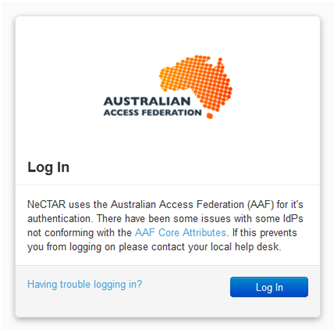
\includegraphics[scale=0.5]{post-workshop/nectar/aaf_login.png}
    \caption{\label{fig:aaf_login}}
  \end{figure}
  \item At the following screen, simply choose your institution from the
  dropdown box and click ``Select". Now follow the on screen prompts and enter
  your regular institutional login details.
  \begin{figure}[H]
    \centering
    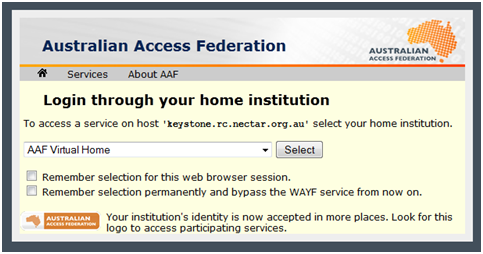
\includegraphics[scale=0.5]{post-workshop/nectar/aaf_home_institute.png}
    \caption{\label{fig:aaf_home_institute}}
  \end{figure}
  \item If you see the following screen, congratulations, you have
  successfully logged into the NeCTAR Research Cloud dashboard!
  \begin{figure}[H]
    \centering
    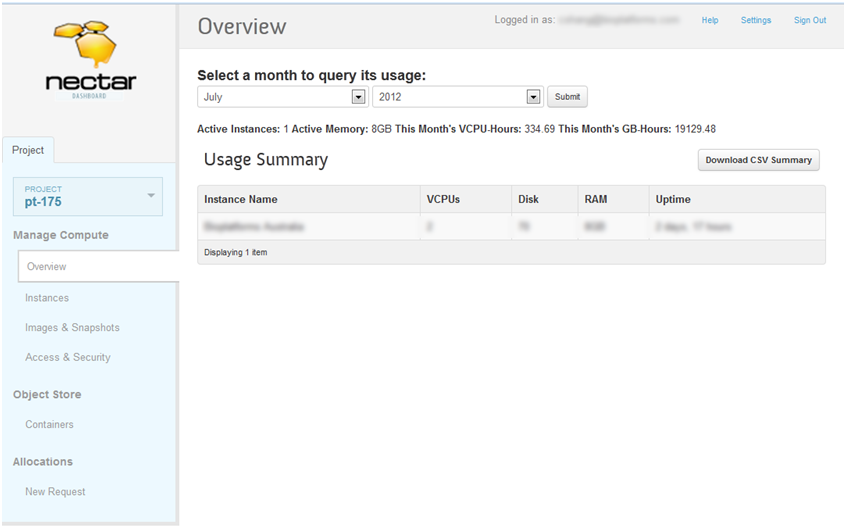
\includegraphics[scale=0.5]{post-workshop/nectar/dashboard_overview.png}
    \caption{\label{fig:dashboard_overview}}
  \end{figure}
\end{enumerate}

\subsubsection{Instantiating Your Own VM}
We will now show you how to instantiate the ``NGS Training'' image using your
own personal cloud allocation.

\begin{enumerate}
  \item In the NeCTAR Research Cloud dashboard, click ``Images \& Snapshots''
  to list all the publicly available images from which you can instantiate a
  VM. Under ``Snapshots" Click the ``Launch" button for the latest version of the
  ``NGSTraining" snapshot:
  \begin{figure}[H]
    \centering
    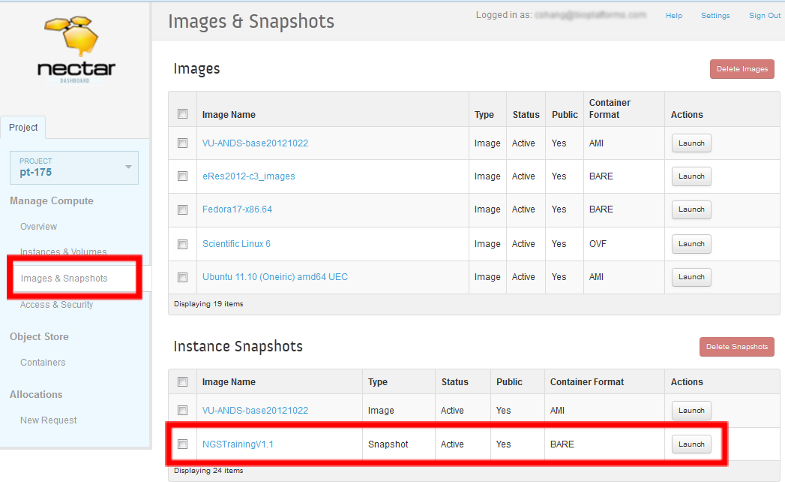
\includegraphics[scale=0.5]{post-workshop/nectar/dashboard_snapshots.png}
    \caption{\label{fig:dashboard_snapshots}}
  \end{figure}
  \item You will now see a ``Launch Instances'' window where you are required to
  enter some details about how you want the VM to be setup before clicking
  ``Launch Instance".
  In the ``Launch Instances'' pop-up frame choose the following settings:
  \begin{description}
  \item[Server Name] A human readable name for your convenience. e.g. ``My NGS VM''
  \item[Flavor] The resources you want to allocate to this VM. I suggest a
  Medium sized VM (2 CPUs and 8 GBytes RAM). This will use all your personal
  allocation, but anything less will probably be insufficient. You could request
  a new allocation of resources if you want to instantiate a larger VM with more
  memory.
  \item[Security Groups] Select SSH.
  \end{description}
  \item Click the ``Launch Instance'' button
  \begin{figure}[H]
    \centering
    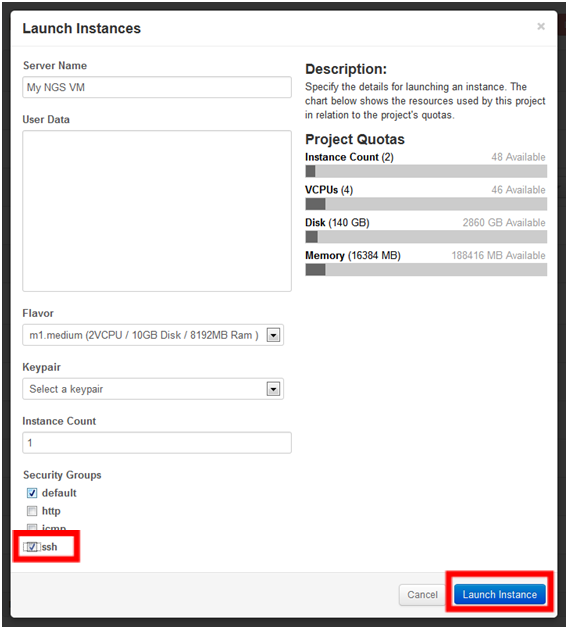
\includegraphics[scale=0.5]{post-workshop/nectar/dashboard_launch.png}
    \caption{\label{fig:dashboard_launch}}
  \end{figure}
  \item You will be taken to the ``Instances" page and you will see the
  ``Status" and ``Task" column for your new VM is ``Building" and ``Spawning". Once
  the ``IP Address" cell is populated, take a note of it as you will need it for
  configuring the NX Client later on.
  \begin{figure}[H]
    \centering
    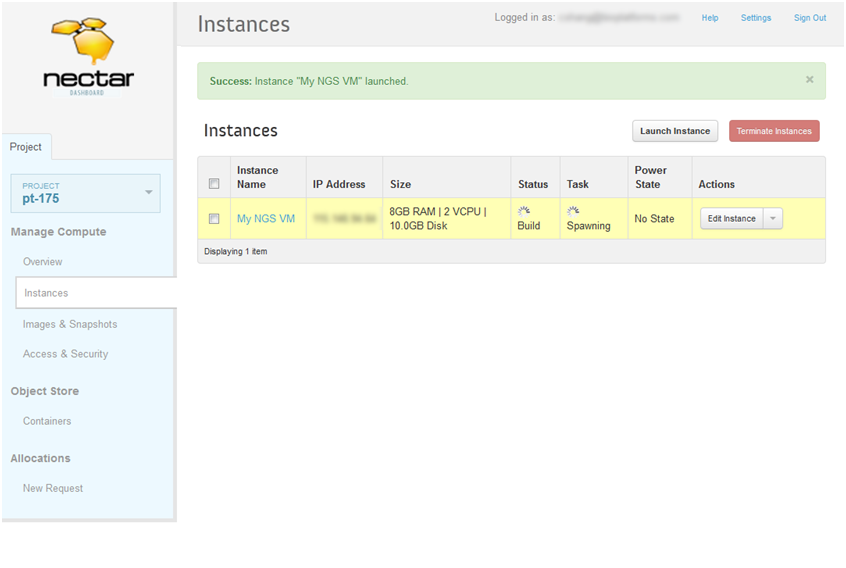
\includegraphics[scale=0.5]{post-workshop/nectar/dashboard_instance_building.png}
    \caption{\label{fig:dashboard_instance_building}}
  \end{figure}
  \item Once the Status and Task for the VM change to ``Active and ``None"
  respectively, your VM is powered up and is configuring itself.
  Congratulations, you have now instantiated a Virtual Machine! If you try to
  connect to the VM too quickly, you might not be successful. The OS may still
  be configuring itself, so give it a few minutes to finish before continuing.
  \begin{figure}[H]
    \centering
    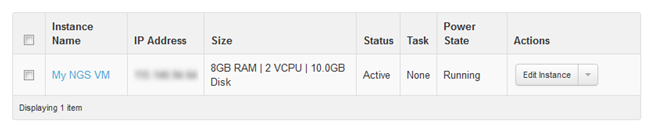
\includegraphics[scale=0.5]{post-workshop/nectar/dashboard_instance_running.png}
    \caption{\label{fig:dashboard_instance_running}}
  \end{figure}
\end{enumerate}

\subsubsection{VM Stuck Building and Spawning}
Sometimes, the cloud experiences a ``hiccup" and a newly instantiated VM will get
stuck in the ``Build" and ``Spawning" state (step 3) for more than a few minutes.
This can be rectified by terminating the instance and creating a new VM from
scratch:
\begin{enumerate}
  \item Selecting ``Terminate Instance" under the ``Edit Instance" dropdown box:
  \begin{figure}[H]
    \centering
    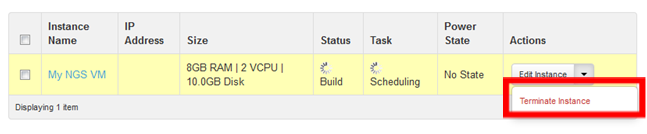
\includegraphics[scale=0.5]{post-workshop/nectar/dashboard_terminate_stuck_instance.png}
    \caption{\label{fig:dashboard_terminate_stuck_instance}}
  \end{figure}
  \item Go back to step 1 of ``Instantiating Your Own VM" and create the VM from scratch:
\end{enumerate}
  

\subsection{Remote Desktop with the NoMachine NX Client}
During the workshop you were using the free NX client from NoMachine
(\url{http://www.nomachine.com/}) to provide a remote desktop-like connection to
VMs running on the NeCTAR Research Cloud. Therefore, we provide information on how to
setup your local computer to connect to the VM you just instantiated in the steps
above.

We assume that:
\begin{itemize}
\item You have administrator rights on your local computer for installing
software.
\end{itemize}

\subsubsection{NoMachine NX Client Installing}
We show you instructions below for the MS Windows version of the NX Client, but
procedures for other supported OSes (Linux, Mac OSX and Solaris) should be very
similar.
\begin{enumerate}
  \item Go to the NoMachine download page: \url{http://www.nomachine.com/download.php}
  \item Click the download icon next to the NX Client for Windows:
  \begin{figure}[H]
    \centering
    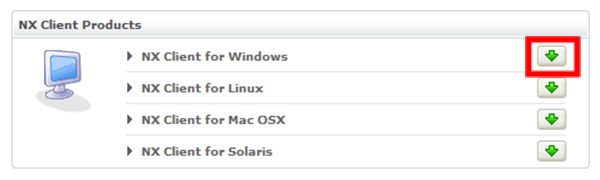
\includegraphics[scale=0.5]{post-workshop/nx_client/download.png}
    \caption{\label{fig:nx_download}}
  \end{figure}
  \item On the "NX Client for Windows" page, click the "Download package" button:
  \begin{figure}[H]
    \centering
    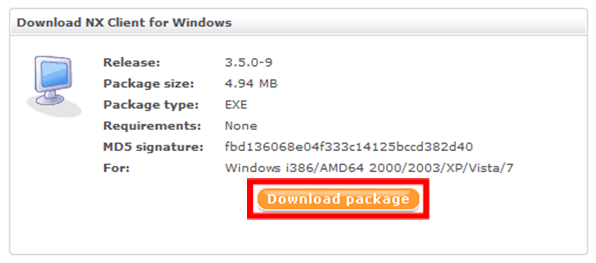
\includegraphics[scale=0.5]{post-workshop/nx_client/download_package.png}
    \caption{\label{fig:nx_download_package}}
  \end{figure}
  \item Run the file you just downloaded (accepting defaults is fine)
  \item Congratulations, you just installed the NoMachine NX Client!
\end{enumerate}

\subsection{NoMachine NX Client Configuration}
Now we have the NoMachine NX Client installed, we need to configure a new NX
"session" which will point to the VM we instantiated in the NeCTAR Research
Cloud.

We assume that:
\begin{itemize}
\item You know the IP address of the VM you want to remote desktop into.
\end{itemize}

\begin{enumerate}
  \item Start the NX Connection Wizard and click "Next" to advance to the
  "Session" settings page.
  \begin{figure}[H]
    \centering
    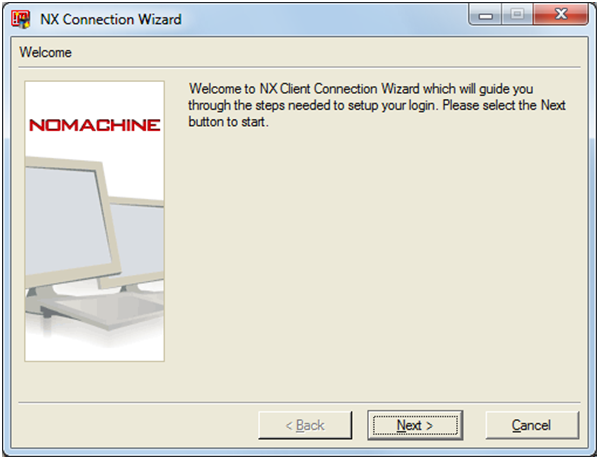
\includegraphics[scale=0.5]{post-workshop/nx_client/start_wizard.png}
    \caption{\label{fig:nx_start_wizard}}
  \end{figure}
  \item On the "Sessions" settings page enter the following details:
  \begin{description}
  \item[Session] A memorable name so you know which VM this session is pointing
  at. You could use the same name you chose for the VM you instantiated earlier
  e.g. "NGS Training".
  \item[Host] Enter the IP address of the VM you instantiated on the NeCTAR
  Research Cloud.
  \begin{figure}[H]
    \centering
    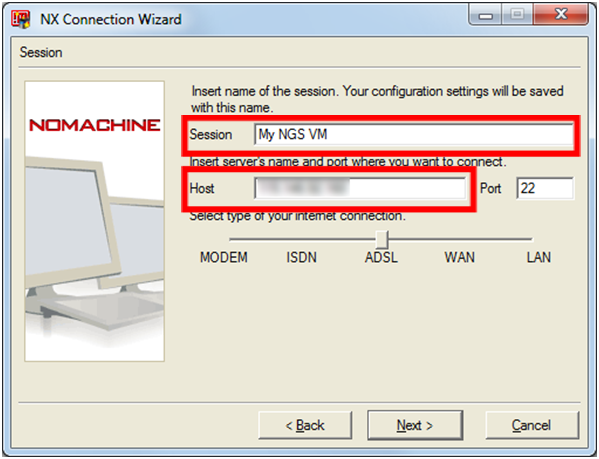
\includegraphics[scale=0.5]{post-workshop/nx_client/session_configuration.png}
    \caption{\label{fig:nx_session_configuration}}
  \end{figure}
  \end{description}
  \item Click "Next" to advance to the "Desktop" settings page. You should use the
  "Unix GNOME" setting.
  \begin{figure}[H]
    \centering
    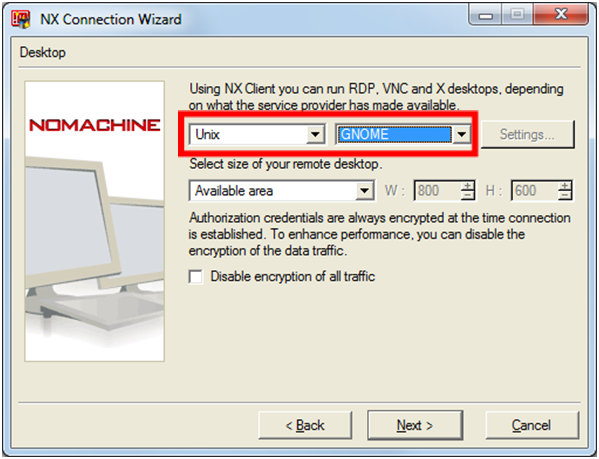
\includegraphics[scale=0.5]{post-workshop/nx_client/desktop_type.png}
    \caption{\label{fig:nx_desktop_type}}
  \end{figure}
  \item Click "Next" and "Finish" to complete the wizard.
\end{enumerate}

\subsection{Connecting to a VM}
If you just completed the NX Connection Wizard described above, the wizard
should have opened the NX Client window. If not, run the "NX Client". You will
be presented with a window like this:
\begin{figure}[H]
  \centering
  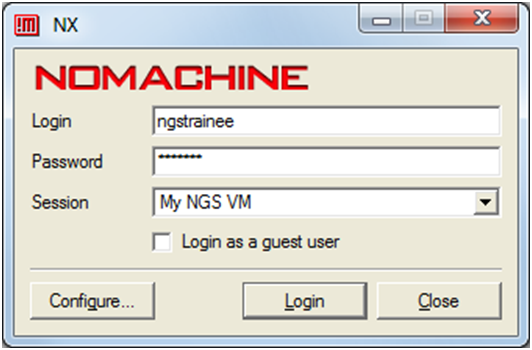
\includegraphics[scale=0.5]{post-workshop/nx_client/login.png}
  \caption{\label{fig:nx_login}}
\end{figure}

The "Login" and "Password" boxes in the NX Client are for user accounts setup on
the VM. By default our image, from which you instantiated your VM, has two
preconfigured users:
\begin{figure}[H]
  \centering
  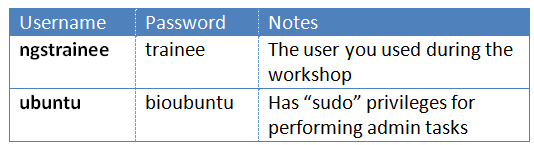
\includegraphics[scale=0.5]{post-workshop/nx_client/usernames_passwords.png}
  \caption{\label{fig:nx_usernames_passwords}}
\end{figure}

Unless you know what you are doing, we suggest you use the \texttt{ngstrainee}
user account details to initiate an NX connection to your VM. In less than a
minute, you should see an NX Window showing the desktop of your VM:
\begin{figure}[H]
  \centering
  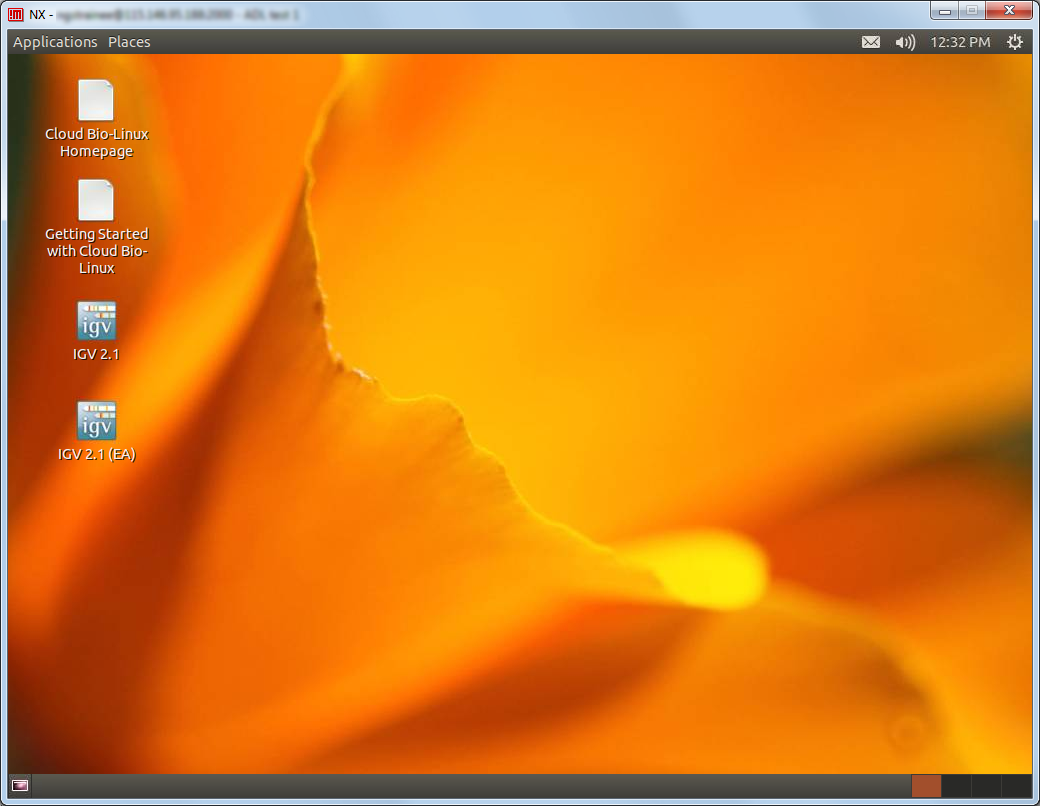
\includegraphics[width=0.8\textwidth]{post-workshop/nx_client/connected.png}
  \caption{\label{fig:nx_connected}}
\end{figure}

\subsection{NX Connection Failure}
In the event that you don't get the NX Window with your VM's desktop displaying
inside it. The most common errors are:
\begin{itemize}
\item You failed to select the "ssh" security group when instantiating the VM.
You'll need to terminate the instance and create a new VM from scratch
\item You failed to select "Unix GNOME" when you configured the NX Client
session. You'll need to reconfigure the session using the NX Client
\item Your institutions firewall blocks TCP port 22. You may need to request this
port to be opened by your local network team or configure the NX client to use a
proxy server.
\end{itemize}

\subsection{Advanced Configuration}
In the session configuration, you can configure the size of the NX Window in
which the desktop of the VM is drawn:
\begin{figure}[H]
  \centering
  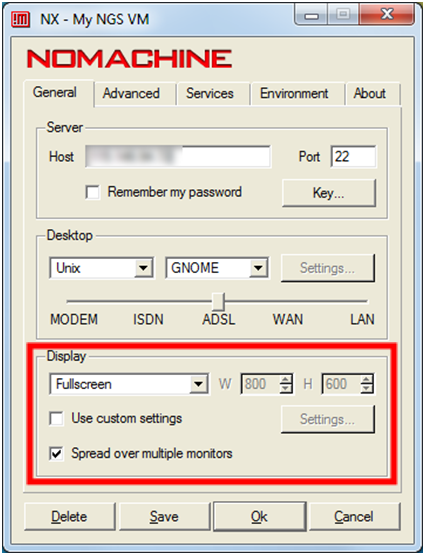
\includegraphics[scale=0.5]{post-workshop/nx_client/advanced_display.png}
  \caption{\label{fig:nx_advanced_display}}
\end{figure}

This can be useful if you want to:
\begin{itemize}
\item Have the NX Window occupy the entire screen, without window decorations.
This is often desirable if you wish to "hide" the host OS from the person
sitting at the computer running the NX Client.
\item Have the NX Window spread over multiple monitors.
\end{itemize}


\clearpage

%
% Access to Workshop Documents
%
\section{Access to Workshop Documents}

This document has been written in \LaTeX\ and deposited in a public github
repository (\url{https://github.com/nathanhaigh/ngs_workshop}). The
documentation has been released under a Creative Commons Attribution 3.0
Unported License (see the Licence page at the beginning of this handout).

For convienience, you can access up-to-date PDF versions of the \LaTeX\ documents at:
\begin{description}[style=multiline,labelindent=0cm,align=left,leftmargin=0.5cm]
\item[Trainee Handout]\hfill\\
\url{https://github.com/downloads/nathanhaigh/ngs_workshop/trainee_handout_latest.pdf}
\item[Trainer Handout]\hfill\\
\url{https://github.com/downloads/nathanhaigh/ngs_workshop/trainer_handout_latest.pdf}
\end{description}

\section{Access to Workshop Data}
Once you have created a VM from our image file, either locally using VirtualBox
or on the NeCTAR Research Cloud, you can configure the system with the workshop
documents and data. This way you can revisit and work through this workshop in
your own time.

In order to do this, we have provided you with access to a shell script which
should be executed on your NGS Training VM by the \texttt{ubuntu} user. This pulls
approx. 3.3 GBytes of data from the NeCTAR Cloud storage and configures the system
for running this workshop:

% NOTE This bash script could be entered into the user data when instantiating
% the VM in the first place
\begin{lstlisting}
# As the ubuntu user run the following commands:
cd /tmp
wget https://github.com/nathanhaigh/ngs_workshop/raw/master/\
workshop_setup/setup_NGS_workshop.sh
bash setup_NGS_workshop.sh
\end{lstlisting}

While you're at it, you may also like to change the timezone of your VM to match
that of your own. To do this simply run the following commands as the
\texttt{ubuntu} user:
\begin{lstlisting}
TZ="Australia/Adelaide"
echo "$TZ" | sudo tee /etc/timezone
sudo dpkg-reconfigure --frontend noninteractive tzdata
\end{lstlisting}

For further information about what this script does and possible command line
arguments, see the script's help:
\begin{lstlisting}
bash setup_NGS_workshop.sh -h
\end{lstlisting}


For further information about setting up the VM for the workshop, please see:
\\\\
\url{https://github.com/nathanhaigh/ngs_workshop/blob/master/workshop_setup/README.md}


\chapter{Space for Personal Notes or Feedback}
\clearpage

%
% Some empty ruled comments pages
%
\myruledpage{3cm}{1cm}
\myruledpage{3cm}{1cm}
\myruledpage{3cm}{1cm}
\myruledpage{3cm}{1cm}

\end{document}
